\chapter{Histórico}
\label{cap:historico}
\section{Primórdios}
Veículos Terrestres não tripulados datam do inicio do século XX, onde em 1921 uma das primeiras aparições de um veículo desse tipo é relatada. A ideia inicial era de que a tecnologia poderia ser adaptada a tanques de guerra. O veículo consistia de um chassi de 3 rodas com um motor e era controlado via rádio. Entre as décadas de 30 e 40, a União das Repúblicas Socialistas Soviéticas, bem como a Alemanha e o Reino Unido criaram versões e seus tanques operados remotamente, com os russos utilizando as suas versões no fronte contra a Finlândia.
\begin{figure}[!htb]
    \centering
    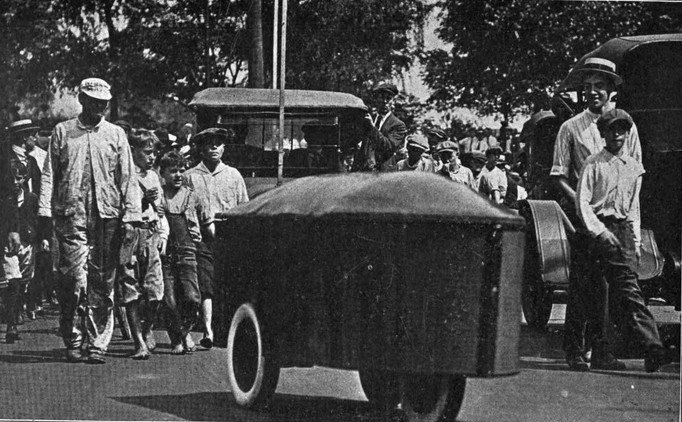
\includegraphics[width=0.75\textwidth]{figuras/controaldo_1921.jpg}
    \caption{Veículo controlado por radio em 1921}
    \label{fig:veiculo:1921}
\end{figure}

Ainda na década de 1940, os alemães criaram um pequeno veículo que utilizava lagartas para se mover para carregar explosivos até as posições inimigas. A inspiração veio de um projeto criado por Adolphe Kegresse encontrado depois da invasão a França. O projeto foi melhorado pelos alemães, recebendo o nome de \textit{Leichter Ladungsträger Goliath}, em português: carregador leve de carga Goliath. Esse pequeno veículo era capaz de carregar uma ogiva de 60kg de explosivos a uma distância de 650 metros. O controle era feito através de um cabo conectado a traseira do veículo. 
\begin{figure}[!htb]
    \centering
    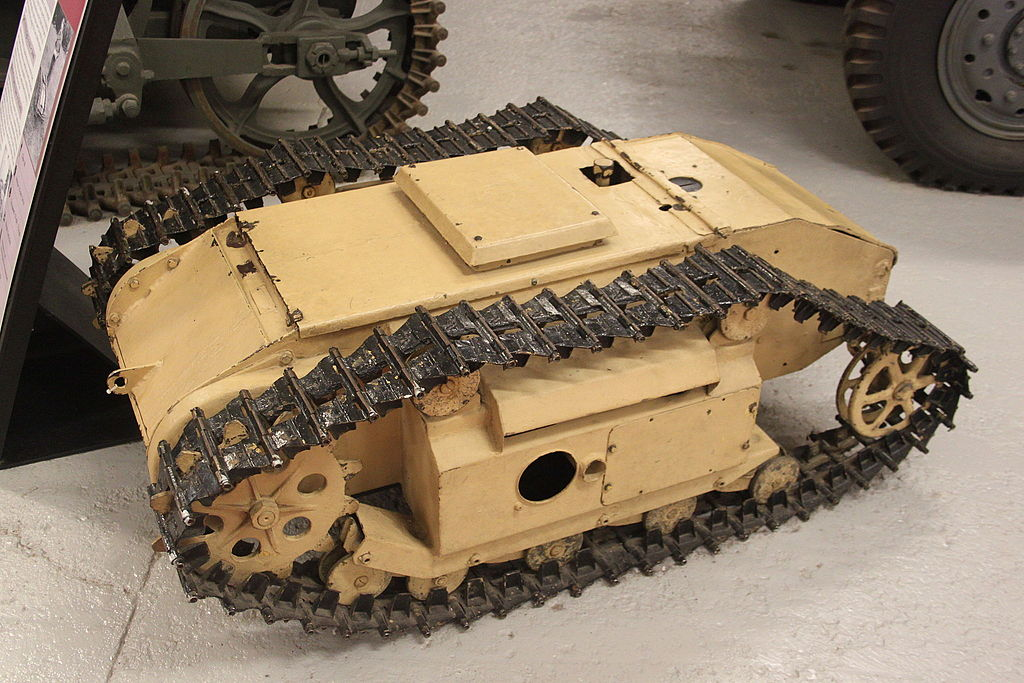
\includegraphics[width=0.75\textwidth]{figuras/goliath.JPG}
    \caption{Um exemplar do Goliath no museu de Tanques de Bovington}
    \label{fig:goliath:museu}
\end{figure}
Cerca de 7564 Goliaths foram construídos, contudo a utilização o mesmo foi limitado, dada a fragilidade do cabo de controle, além disso, a complexidade da sua manutenção no campo de batalha era grande, isso somadas a baixa velocidade, blindagem de apenas 10mm e o peso, considerado muito grande para ser facilmente transportado.
\section{Inicio da automação}
Na década de 60 surgiu o Shakey, o primeiro robô autônomo criado por Charles Rosen com fundos provenientes da Agência de Projetos de Pequisa Avançada de Defesa(Defense Advanced Research Projects Agency - D.A.R.P.A). Shakey conseguia perceber o espaço e depois da análise do ambiente, criar um plano de ação para realizar um número de ações. 

\begin{figure}[H]
    \centering
    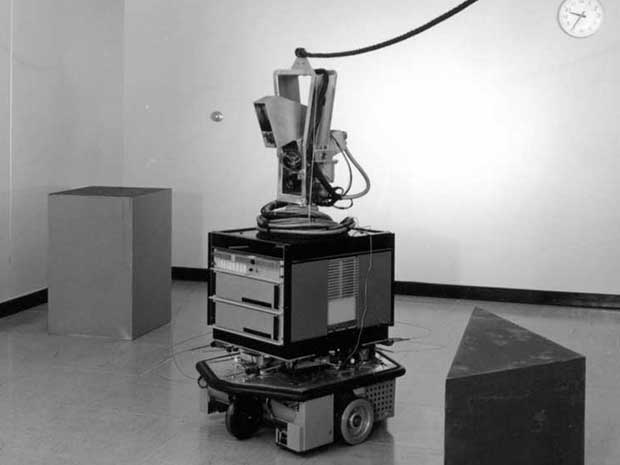
\includegraphics[width=0.75\textwidth]{figuras/shakey_robot.jpeg}
    \caption{Shakey, o robô. Seu nome vem do fato e chacoalhar muito durante sua movimentação}
    \label{fig:shakey:robo}
\end{figure}

A pesquisa de Shakey culminou em um grande impacto sentido em vários campos de pesquisa, tais como robótica e inteligência artificial, bem como a ciência da computação em si. A pesquisa resultou no algoritmo de pesquisa A* usado para achar caminhos e transversais de grafos. Além de avanços no processamento de imagens, visão computacional e análise de imagens\cite{cassel:2017}.

Já na década de 1970, a empresa Pyxus colocou no mercado o robô HelpMate desenhado a executar tarefas dentro de um hospital. Partindo do pressuposto de que tarefas de que "transporte" tomavam um tempo essencial dos enfermeiros e de que na época existia uma demanda desses profissionais, a ideia de criar um sistema que pudesse suprir essa demanda foi explorada. De forma autônoma, HelpMate, percorria o hospital mostrando um comportamento humanizado carregando refeições, suprimentos estéreis, medicações, registros médicos, amostras e cartas\cite{evans:1992}. Ele conseguia se movimentar pelo hospital graças a mapas pré-carregados em seu sistema. Além disso, era dotado de sonares, infravermelho e detectores de colisão.
\begin{figure}[H]
    \centering
    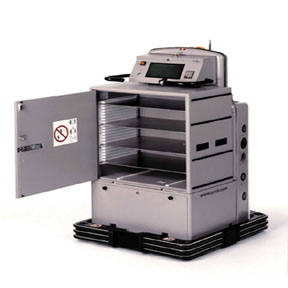
\includegraphics[width=0.75\textwidth]{figuras/helpmate.jpg}
    \caption{HelpMate, robô para auxiliar em atividades de transporte em hospitais}
    \label{fig:helpmate:robo}
\end{figure}

HelpMate conseguia 98\% de sucesso em suas missões, logando em seus sistemas os sucessos e também os  motivos por uma possível falha. Ficou claro que as falhas catalogadas eram provenientes de erros do usuário ou de forças externas a suas capacidades, como tarefas agendadas de forma errônea, falhas em elevadores ou paradas emergências e não por falhas de \textit{hardware} ou incapacidade de navegar até seus objetivos.

A CyberMotion criou por sua vez o SR2, um robô de 3 rodas para segurança de instalações equipado com um sistema e navegação ultrassônico e um sistema anticolisão, além disso, era equipado com sensores de umidade, fogo, fumaça ou gases, podia detectar movimento e avisar caso percebesse um intruso. Contudo, a empresa falhou em fazer o produto vender, fechando as portas em 2005 \cite{bracht:2015}.
\begin{figure}[H]
    \centering
    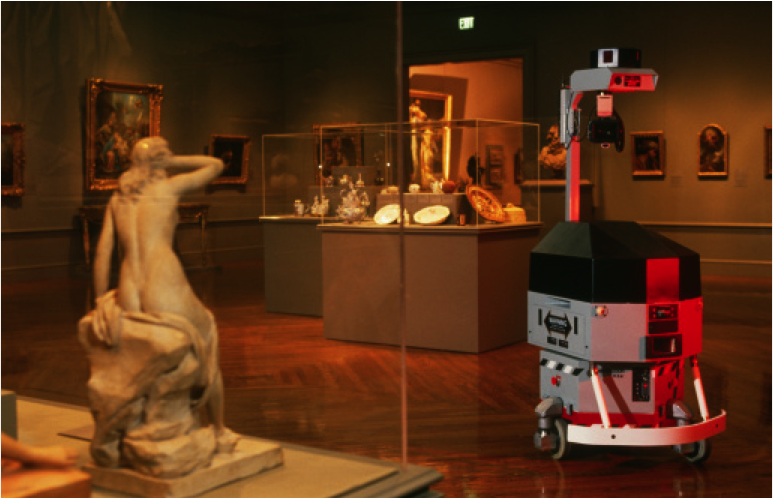
\includegraphics[width=0.75\textwidth]{figuras/cybermotion SR2.png}
    \caption{Robô de segurança SR2 da CyberMotion}
    \label{fig:cybermotion:sr2}
\end{figure}


\section{Aplicação na agricultura}
Em 2016 na \textit{Farm Progress Show} no estado de Iowa foram apresentados pela \textit{CNH Industrial} dois protótipos de tratores autônomos: o \textit{Case IH Magnum} e o \textit{New Holland T8 NHDrive}. Apesar de tecnologias capazes de controlar certos aspectos da operação de um trator já existirem, como direção automática e correção de direção por GPS, as empresas foram além, criando sistemas autônomos capazes de operar por completo os tratores. Já que são baseados em tratores já existentes, a maioria de componentes convencionais foram mantidos como motores, transmissões, chassi e módulos de acoplagem e no caso do \textit{T8 NHDrive}, a cabine do operador foi mantida por questões operacionais\cite{engineer:2016}.

A \textit{Jacto} por sua vez vem trabalhando no seu próprio veiculo aqui no Brasil, o \textit{Jacto Autonomous Vehicle}, desde 2008. O \textit{JAV} é capaz de operar na lavoura por horas sem intervenção humana, sendo capaz também de trocar informações e dividir o trabalho entre outros veículos que estejam na mesma área\cite{jacto:2018}. Até o momento o JAV é apresentado na versão de pulverização, mas os projetos podem ser modificados no futuro para que possa receber outras funções.

\begin{figure}[H]
    \begin{center}
    % jacto
        \subfigure[]{
            \label{Jacto:jav}
            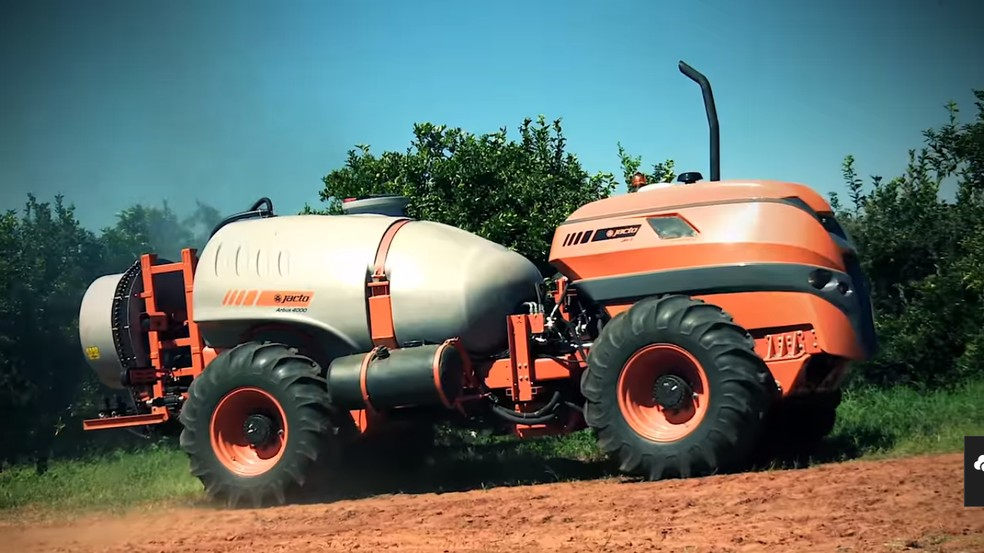
\includegraphics[width=0.4\textwidth]{figuras/jacto-jav.png}
        }
        % new holland
        \subfigure[]{
            \label{Holland:T8}
            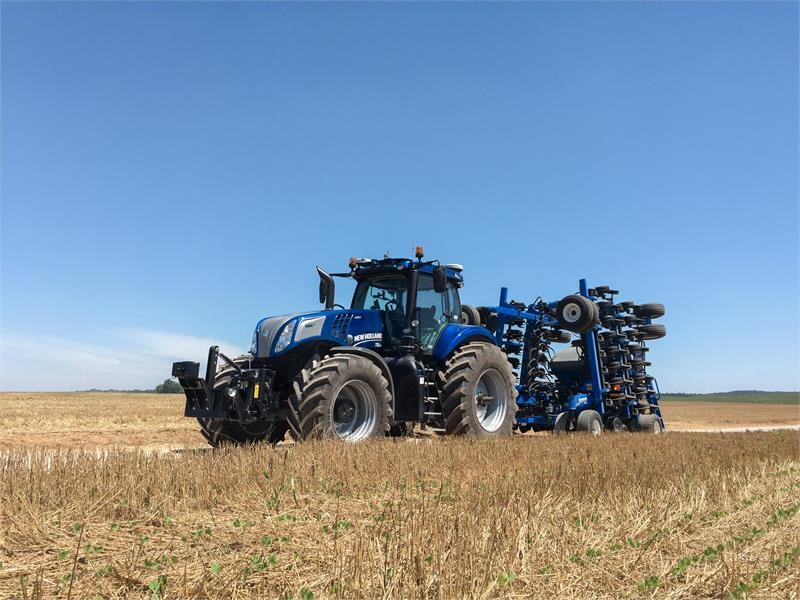
\includegraphics[width=0.4\textwidth]{figuras/newhollandt8.png}
        }
           % CASE
        \subfigure[]{
            \label{Case:Magnum}
            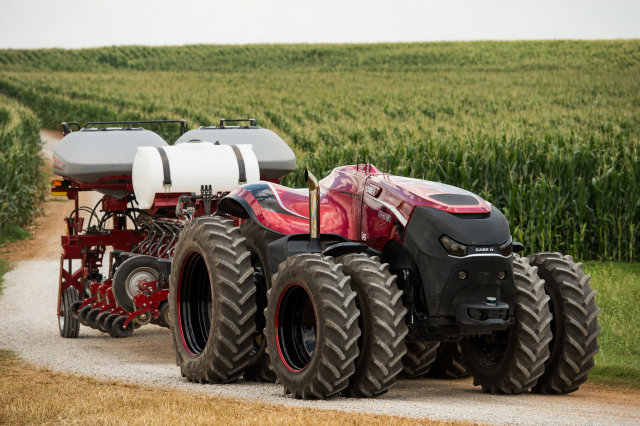
\includegraphics[width=0.4\textwidth]{figuras/CaseMagnum.jpg}
        }
    \end{center}
    \caption{%
        (a) Jacto JAV II, (b) New Hollando T8 NHDrive, (c) Case IH Magnum
     }%
\end{figure}


Os três veículos, apesar de implementados de forma diferente, operam similarmente: um plano de trabalho é criado baseado em uma área pré-estabelecida através de coordenadas GPS, após isso, um sistema calcula a melhor rota a ser seguida, levando em consideração consumo de combustível, obstáculos, o tamanho dos implementos agrícolas\footnote{Implementos agrícolas são apetrechos que são necessários para desempenhar uma certa ação. Exemplo: arados, plantadoras, niveladoras} acoplados e outras máquinas operando na vizinhança. Caminhos podem ser inseridos manualmente caso seja necessário. Todo esse sistema pode ser controlado via dispositivo móvel ou em um computador, onde também serão mostrados os caminhos a serem tomados, bem como o progresso da operação, além de opções para modificação dos parâmetros de operação dos implementos.

Para tais missões, as máquinas são dotadas dos mais diversos sensores, passando de várias câmeras, microfones, sensores de proximidade e até mesmo radares. Com esse vasto arsenal possibilita-se que o sistema tome decisões durante sua missão, tais como evitar obstáculos ou colisões. Dado o nível de autonomia das mesmas é possível que um operador seja capaz de gerenciar N veículos com diferentes funções, acompanhando o progresso de cada uma e ajustando os parâmetros se necessário.
